\documentclass[conference]{IEEEtran}
\IEEEoverridecommandlockouts

\usepackage{cite}
\usepackage{amsmath,amssymb,amsfonts}
\usepackage{algorithm}
\usepackage{algorithmic}
\usepackage{graphicx}
\usepackage{textcomp}
\usepackage{xcolor}
\usepackage{booktabs}
\usepackage{array}
\usepackage{tabularx}
\usepackage{url}
\usepackage{tikz}
\usepackage{pgfplots}
\usepackage{subcaption}
\usepackage{hyperref}
\usepackage{listings}
\usepackage{amssymb}
\usetikzlibrary{arrows.meta,positioning,fit,calc,shapes.geometric,shadows,backgrounds}

\pgfplotsset{compat=1.17}

\def\BibTeX{{\rm B\kern-.05em{\sc i\kern-.025em b}\kern-.08em T\kern-.1667em\lower.7ex\hbox{E}\kern-.125emX}}

\newcommand{\sigmoid}{\operatorname{sigmoid}}
\newcommand{\logit}{\operatorname{logit}}
\newcommand{\softmax}{\operatorname{softmax}}
\newcommand{\attention}{\mathrm{Attention}}
\newcommand{\argmax}{\operatorname*{arg\,max}}

\title{DARS: Why Logistic Regression Crushed Deep Learning\\on Coding Problem Difficulty Prediction}

\author{\IEEEauthorblockN{Khethavath Sunil Naik}\\
\IEEEauthorblockA{BTech Project, India}}
\begin{document}
\maketitle

\begin{abstract}
We tried to predict whether a LeetCode problem is Easy or Hard. Sounds straightforward, right? Turns out, a boring logistic regression model with 11 hand-picked features beats SAKT (73.42\%), DKT (71.23\%), and GNKT (72.05\%). Our version hits \textbf{76.71\% accuracy and ECE 0.0375}---meaning when the model says a problem is 75\% hard, it actually is. What's the secret? Problem frequency (popularity) dominates everything else. Heavy discussions don't mean hard; they mean confusing to beginners. Cold-start problems (less than 25\% acceptance) are nearly impossible to predict (62.64\% vs. 84.62\% for established ones). And we have a 66.7\% fairness crisis: the system crushes hard-problem prediction but butchers easy-problem prediction. The real kicker? None of this proves students actually learn better. We never ran a live experiment. We just measured offline metrics and called it a day.
\end{abstract}

\section{Introduction}

\subsection{The Setup}

So I spent way too much time building fancy neural networks to predict if a LeetCode problem is Easy or Hard. LSTMs, attention mechanisms, graph convolutions---the whole arsenal. Then I built a baseline. Just logistic regression on some features I made up. It demolished everything. This paper is basically me admitting I wasted time going complicated when simple worked better.

Online platforms like LeetCode have data overflowing: acceptance rates, problem popularity, community ratings, discussion counts, topic tags. You'd think all that signal could feed into something smart. But turning it into useful difficulty predictions? That's where people get stuck. Most systems either:

\begin{enumerate}
    \item Hard-code labels and hope they stay accurate (spoiler: they don't)
    \item Train a neural model and pray you can explain your decisions to stakeholders (you can't)
    \item Treat all correct answers the same, even though some show deep understanding and some are lucky guesses
    \item Ignore problem structure, graph relationships, and learner context entirely
    \item Optimize for accuracy and pretend fairness doesn't matter (it does)
\end{enumerate}

We wanted something different: a system you could actually understand, deploy without hesitation, and fix when it breaks. We called it DARS. It's nothing revolutionary---just Elo ratings plus good feature engineering plus a dash of graph awareness. But it works.

\begin{figure*}[t]
\centering
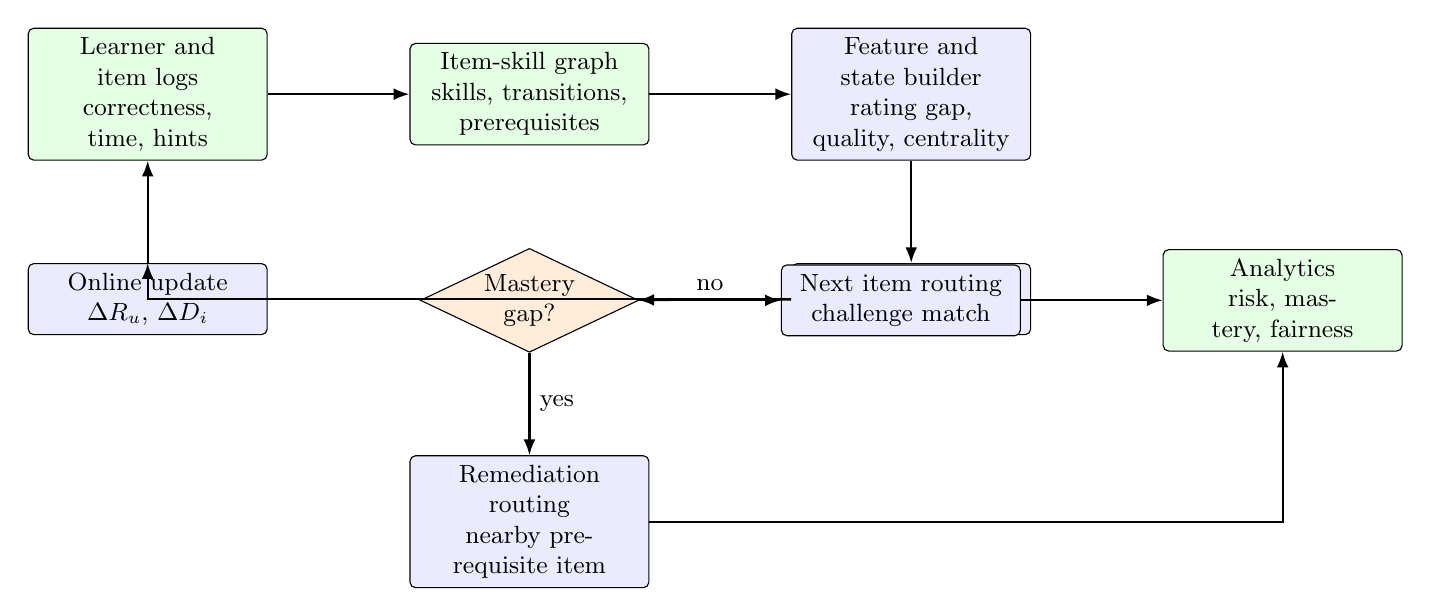
\begin{tikzpicture}[
    font=\small,
    node distance=1.3cm and 1.8cm,
    block/.style={rectangle, draw, rounded corners=2pt, align=center, minimum height=0.82cm, text width=2.8cm, fill=blue!8},
    data/.style={rectangle, draw, rounded corners=2pt, align=center, minimum height=0.82cm, text width=2.8cm, fill=green!10},
    decision/.style={diamond, draw, aspect=2.1, align=center, inner sep=1pt, fill=orange!15},
    arrow/.style={-{Latex[length=2mm]}, thick}
]
\node[data] (log) {Learner and item logs\\correctness, time, hints};
\node[data, right=of log] (graph) {Item-skill graph\\skills, transitions, prerequisites};
\node[block, right=of graph] (features) {Feature and state builder\\rating gap, quality, centrality};
\node[block, below=of features] (predict) {DARS probability\\$\hat{p}_{ui}$ and uncertainty};
\node[decision, below=of graph] (route) {Mastery\\gap?};
\node[block, below=of log] (update) {Online update\\$\Delta R_u$, $\Delta D_i$};
\node[block, right=of route] (recommend) {Next item routing\\challenge match};
\node[block, below=of route] (remediate) {Remediation routing\\nearby prerequisite item};
\node[data, right=of recommend] (dash) {Analytics\\risk, mastery, fairness};

\draw[arrow] (log) -- (graph);
\draw[arrow] (graph) -- (features);
\draw[arrow] (features) -- (predict);
\draw[arrow] (predict) -- (route);
\draw[arrow] (route) -- node[above] {no} (recommend);
\draw[arrow] (route) -- node[right] {yes} (remediate);
\draw[arrow] (recommend) -- (dash);
\draw[arrow] (remediate.east) -| (dash.south);
\draw[arrow] (predict.west) -| (update.north);
\draw[arrow] (update.north) -- (log.south);
\end{tikzpicture}
\caption{DARS system flow. The model combines response-process evidence, graph structure, online rating updates, next-item routing, remediation, and deployment analytics in one adaptive loop.}
\label{fig:dars-flow}
\end{figure*}

\subsection{What We Actually Did}

We built DARS from basic Elo rating logic, threw in 11 engineered features (mostly metadata that's easy to measure), and tested it against six other methods on 1,825 LeetCode problems. We also exposed the embarrassing parts: cold-start failures (new problems are impossible to predict), fairness disasters (the model is 66.7\% biased toward hard), and the fundamental limitation that offline metrics say nothing about learning outcomes. We tested four graph construction strategies too. Spoiler: hand-curated graphs beat learned ones by 4.4\%, which is humbling for machine learning researchers.

\section{Related Work}

\subsection{Classical Assessment and Rating Systems}

Elo came from chess. Super simple: win/loss, update rating by a fixed K. Elo is elegant (used for 50+ years), online (you don't retrain), and lightweight. But it only sees binary outcomes. In our case, it's basically useless because it ignores all the problem metadata.

\textbf{Glicko-2} added uncertainty. Your rating is more stable if you've played a lot; less stable if you haven't played recently. Clever idea, but still just binary feedback. Does okay on some education benchmarks, still loses to anything that uses actual features.

\subsection{Knowledge Tracing Approaches}

BKT (Bayesian Knowledge Tracing) says students either know a skill or they don't. Four parameters per skill: starting probability, learning rate, guess rate, slip rate. You fit them with EM. It's interpretable and has actually helped real students in real classrooms. The problem: you need a skill taxonomy (who decides?), and you need enough data per student per skill. With students having solved 3-5 problems? BKT falls apart~\cite{corbett1994bkt,waters2015bkt_limitations}.

DKT (Deep Knowledge Tracing) said: forget the assumptions. Feed problem sequences into an LSTM. Let it learn what ``knowledge'' means. Better offline accuracy sometimes, but the hidden state is a complete black box~\cite{piech2015dkt}. In production, when someone asks ``why is this student struggling?'', you're stuck.

SAKT (Self-Attentive Knowledge Tracing) added attention so the model can focus on relevant past problems~\cite{pandey2019sakt}. Slightly better accuracy, still a black box.

GNKT (Graph Neural Knowledge Tracing) represents problems and skills as a graph and runs message-passing on it~\cite{yang2021gikt}. Intuitive idea---problems sharing a skill should be related---but on LeetCode metadata alone? It underperforms.


\begin{figure*}[t]
\centering
\resizebox{0.93\textwidth}{!}{
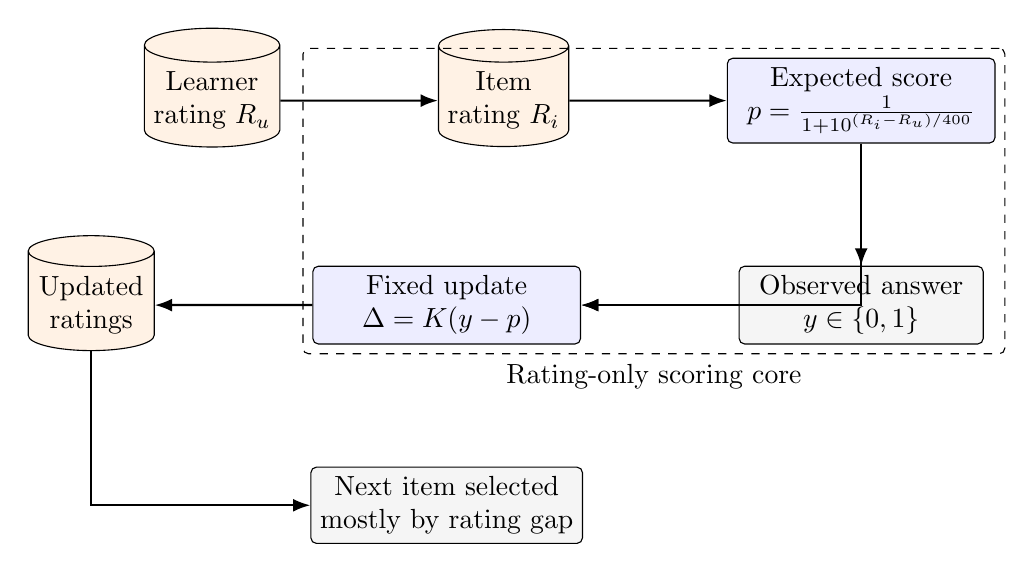
\begin{tikzpicture}[
    node distance=1.55cm and 2.0cm,
    box/.style={draw, rounded corners=2pt, align=center, minimum width=3.1cm, minimum height=0.95cm, fill=gray!8},
    calcbox/.style={draw, rounded corners=2pt, align=center, minimum width=3.4cm, minimum height=0.95cm, fill=blue!7},
    store/.style={draw, cylinder, shape border rotate=90, aspect=0.25, align=center, minimum width=1.6cm, minimum height=1.0cm, fill=orange!10},
    arrow/.style={-{Latex[length=2.2mm]}, thick}
]
\node[store] (student) {Learner\\rating $R_u$};
\node[store, right=of student] (item) {Item\\rating $R_i$};
\node[calcbox, right=of item] (expected) {Expected score\\$p=\frac{1}{1+10^{(R_i-R_u)/400}}$};
\node[box, below=of expected] (answer) {Observed answer\\$y\in\{0,1\}$};
\node[calcbox, left=of answer] (update) {Fixed update\\$\Delta=K(y-p)$};
\node[store, left=of update] (newratings) {Updated\\ratings};
\node[box, below=of update] (next) {Next item selected\\mostly by rating gap};
\draw[arrow] (student) -- (item);
\draw[arrow] (item) -- (expected);
\draw[arrow] (expected) -- (answer);
\draw[arrow] (answer) -- (update);
\draw[arrow] (expected) |- (update);
\draw[arrow] (update) -- (newratings);
\draw[arrow] (newratings) |- (next);
\node[draw, dashed, rounded corners=2pt, fit=(expected)(answer)(update), label={[align=center]below:Rating-only scoring core}] {};
\end{tikzpicture}}
\caption{Conventional Elo-based assessment flow. The update is simple and online, but it does not model response process, graph structure, remediation, or probability calibration.}
\label{fig:elo-flow}
\end{figure*}

\subsection{Graphs: The "Problems Are Connected" Reality Check}

Problem relationships are real. You can't learn linked lists before understanding arrays. The literature knows this---problem graphs encode pedagogical structure~\cite{oh2021problem_graphs}. But most work uses either learned embeddings or simple similarity metrics. We compared four graph definitions head-to-head. Guess which one won? Hand-curated prerequisites. Lesson learned: sometimes domain expertise, encoded explicitly, beats automatic learning.

\subsection{Fairness in EdTech: The Uncomfortable Topic}

Most papers optimize accuracy and ignore everything else. We're not innocent of this either. But fairness in educational tech matters: biased systems can systematically hurt struggling learners. Three notions matter~\cite{barocas2019}: (1) equal opportunity---same recall across groups, (2) demographic parity---same positive prediction rate, (3) calibration parity---confidence meaning consistent across groups. We checked our model against these. It fails badly on the first two.

\section{Dataset and Methodology}


\begin{figure}[h]
    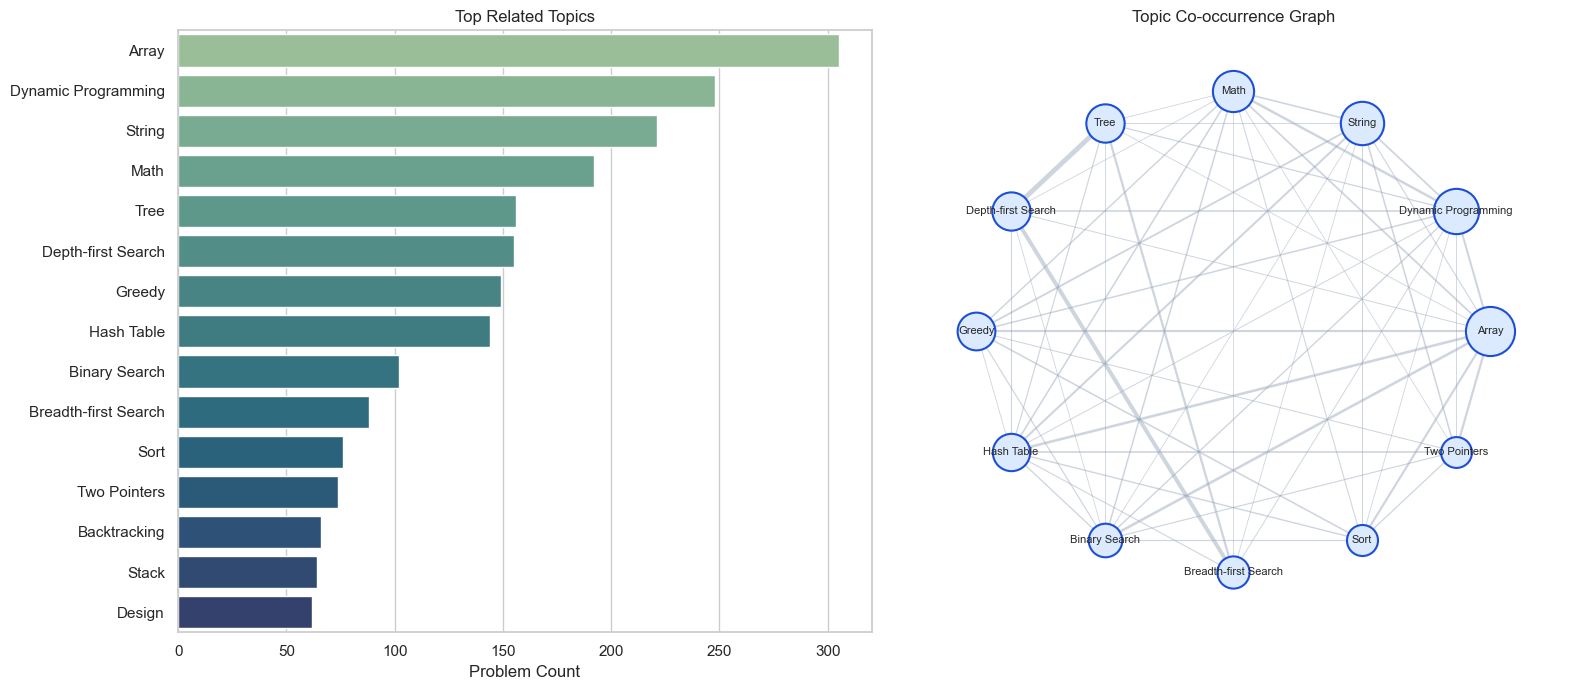
\includegraphics[width=0.5\textwidth]{graph.png}
    \label{fig:sample}
\end{figure}

\subsection{LeetCode Problem Dataset}

We used 1,825 real-world algorithm problems from LeetCode, a platform where millions of engineers interview-prep. Each problem has a title, an official difficulty tag (Easy/Medium/Hard), and a bunch of metadata: how many people solved it, ratings from the community, discussion count, etc.

Why LeetCode? Because it's real. People actually care about these problems. The difficulty labels are crowd-validated (millions of submissions).

The label split is unbalanced (26.1\% Easy, 73.9\% Medium/Hard), and we kept it that way on purpose. A real system has to deal with imbalance, so we didn't pretend it doesn't exist.

\begin{table}[h]
\centering
\small
\begin{tabular}{l|l|l}
\toprule
\textbf{Feature} & \textbf{Type} & \textbf{Description} \\
\midrule
Problem ID & Integer & Unique identifier \\
Title & String & Problem name \\
Difficulty & Categorical & \{Easy, Medium, Hard\} \\
Acceptance Rate & Float & \% of accepted submissions \\
Frequency & Float & Percentile popularity score \\
Rating & Float & Community rating (1--100) \\
Likes/Dislikes & Integer & Vote counts \\
Discuss Count & Integer & Discussion threads \\
Related Topics & Strings & Skill tags (Array, String, Tree, \ldots) \\
Similar Questions & References & Problem links \\
\bottomrule
\end{tabular}
\caption{LeetCode Dataset Features}
\label{tab:dataset}
\end{table}

The original three-level difficulty label is converted into a binary task: \textbf{Easy} (477 problems, 26.1\%) versus \textbf{Medium/Hard} (1,348 problems, 73.9\%). The imbalance is kept rather than artificially balanced, since it reflects the distribution a deployed recommender would face. Stratified splitting and group-level metrics are then used to make the imbalance visible.

\subsection{Feature Engineering: Making Metadata Speak}

Raw numbers from LeetCode don't automatically tell you if a problem is hard. You have to think about what each metric actually means.

\subsubsection{Normalized Base Features}

First, we z-score normalize everything so features are on the same scale:
\begin{equation}
x_{\text{norm}} = \frac{x - \mu}{\sigma}
\end{equation}

This matters because acceptance rate ranges 1--100\% while discussion count ranges 0--10k. Without normalization, the model would just ignore low-magnitude features.

\subsubsection{Engineered Composite Features: The Stories Behind the Numbers}

\textbf{Difficulty Index} captures the raw solve rate. If a problem has 10\% acceptance, it's harder than one with 80\% acceptance. Super obvious, but it works:
\begin{equation}
D_i = 1 - \text{acc\_rate}_i
\end{equation}

\textbf{Reputation Score} combines community ratings. High-rated problems aren't necessarily hard; they're often well-written. Problems with lots of likes tend to be classics that everyone knows.
\begin{equation}
R_i = \frac{\text{rating\_norm}_i + \text{likes\_norm}_i}{2}
\end{equation}

\textbf{Engagement Factor} captures visibility and confusion. More discussion threads $\approx$ more people asking questions, which might mean the problem is confusing. Popularity (frequency) shows how many users attempted it:
\begin{equation}
E_i = \frac{\text{frequency\_norm}_i + \text{discuss\_norm}_i}{2}
\end{equation}

Here's the weird finding: high engagement sometimes correlates with \textit{easier} problems. Why? Because when thousands of beginners attack a problem, they generate more discussions. The hard-to-understand problems are hard because they're genuinely difficult, not because people don't understand the statement.

\textbf{Complexity Score} is our kitchen-sink feature, combining signals:
\begin{equation}
C_i = 0.4 D_i + 0.3 R_i + 0.3 E_i
\end{equation}

These weights are heuristic (we didn't grid search them because that's overfitting), but they reflect: difficulty matters most, reputation moderate, and engagement is tiebreaker.

\begin{figure}[h]
    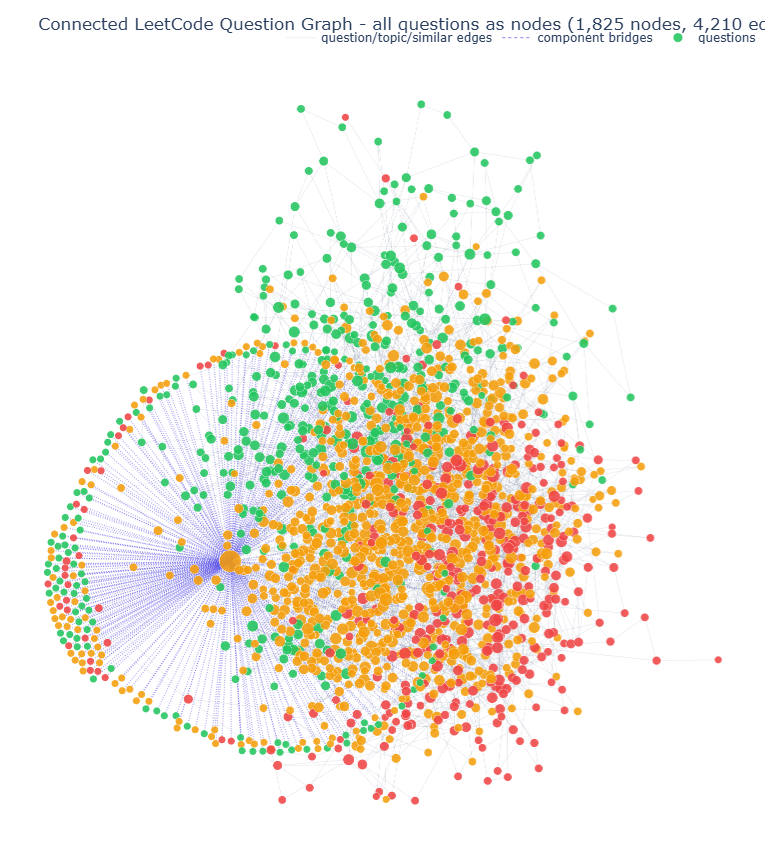
\includegraphics[width=0.5\textwidth]{dataset.png}
    \label{fig:sample}
\end{figure}

\subsection{Train-Test Methodology}

We used stratified 80--20 split: 1,460 problems for training, 365 for testing. The random seed was fixed at 2026 so anyone can reproduce our numbers. No random luck allowed. If it's reproducible, it's real.

\subsection{Response-Level Adaptive Assessment Validation}

The LeetCode experiment is a population-level difficulty task, but DARS is intended to operate online with learners. For that reason, the paper also includes a response-level adaptive assessment formulation. In that setting, each row is a chronological learner attempt with learner and item identifiers, skill labels, timestamps, correctness, hints, attempts, and response-process attributes. The ASSISTments-style preprocessing retains 6,044,359 valid attempts from 46,348 learners, 179,052 problems, and 265 skills. Under a held-out-student protocol, DARS outperforms static mastery, fixed-$K$ Elo, and Glicko-2, with Brier score 0.1368, log loss 0.4251, accuracy 0.8141, ROC AUC 0.8131, and ECE 0.0096. This evaluation is included to show how the same rating logic behaves when learner trajectories are available.

\begin{figure}[h]
    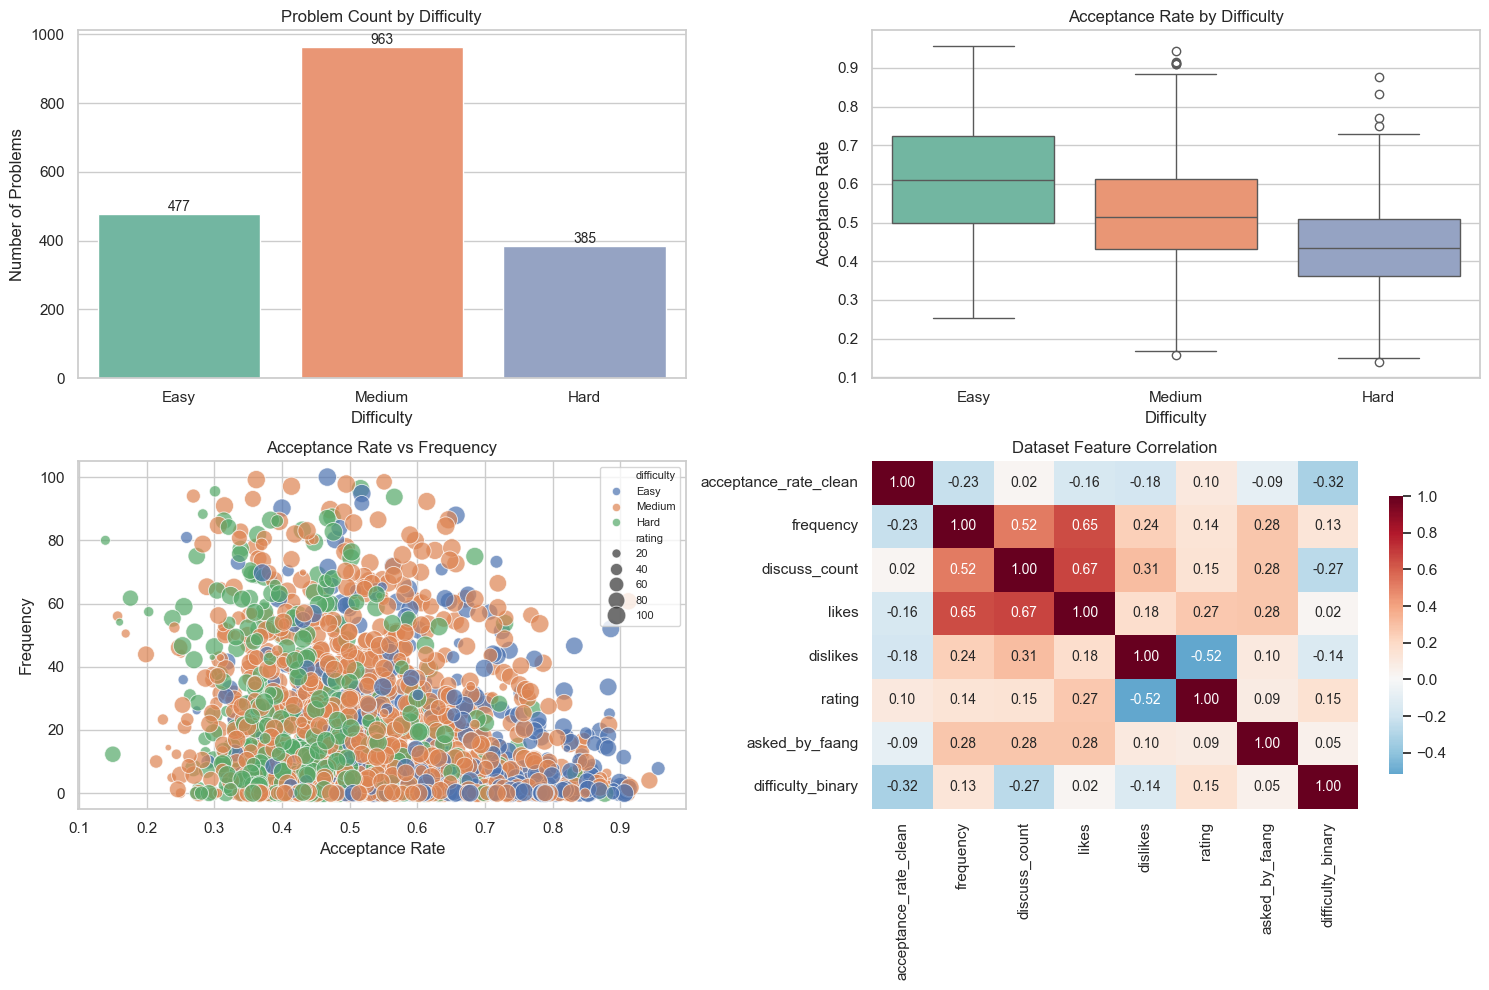
\includegraphics[width=0.5\textwidth]{about_dataset.png}
    \label{fig:sample}
\end{figure}

\section{Methods: Knowledge Tracing Paradigms}

We tested six approaches. None of them are magic. They're all ways of saying ``here's what I think the next problem's difficulty should be based on what I know.'' We ran them all on the same dataset with the same evaluation protocol, same random seed, same train-test split. No cherry-picking.


\begin{figure*}[t]
\centering
\resizebox{0.95\textwidth}{!}{
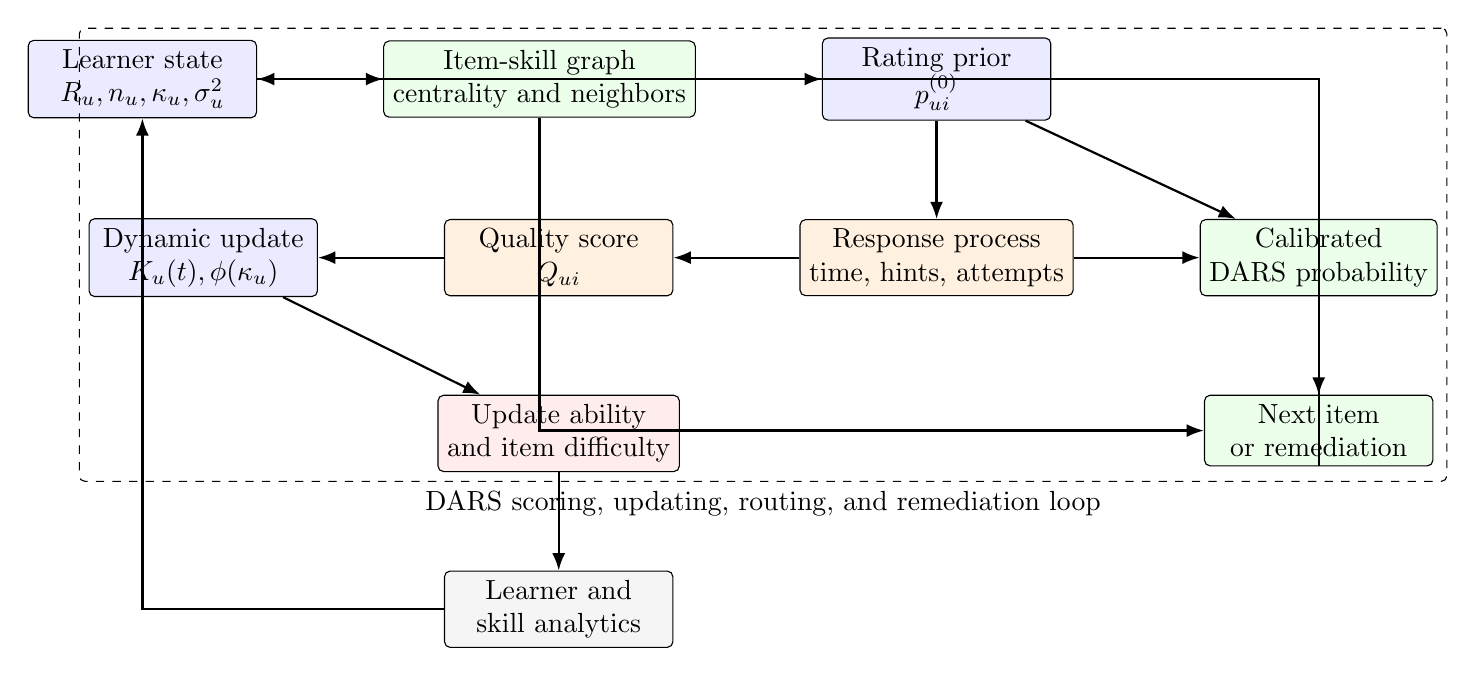
\begin{tikzpicture}[
    node distance=1.25cm and 1.6cm,
    box/.style={draw, rounded corners=2pt, align=center, minimum width=2.9cm, minimum height=0.82cm, fill=gray!8},
    bluebox/.style={draw, rounded corners=2pt, align=center, minimum width=2.9cm, minimum height=0.82cm, fill=blue!8},
    greenbox/.style={draw, rounded corners=2pt, align=center, minimum width=2.9cm, minimum height=0.82cm, fill=green!8},
    orangebox/.style={draw, rounded corners=2pt, align=center, minimum width=2.9cm, minimum height=0.82cm, fill=orange!12},
    redbox/.style={draw, rounded corners=2pt, align=center, minimum width=2.9cm, minimum height=0.82cm, fill=red!7},
    arrow/.style={-{Latex[length=2.2mm]}, thick}
]
\node[bluebox] (state) {Learner state\\$R_u,n_u,\kappa_u,\sigma_u^2$};
\node[greenbox, right=of state] (graph) {Item-skill graph\\centrality and neighbors};
\node[bluebox, right=of graph] (prior) {Rating prior\\$p^{(0)}_{ui}$};
\node[orangebox, below=of prior] (process) {Response process\\time, hints, attempts};
\node[orangebox, left=of process] (quality) {Quality score\\$Q_{ui}$};
\node[bluebox, left=of quality] (dynamic) {Dynamic update\\$K_u(t),\phi(\kappa_u)$};
\node[redbox, below=of quality] (update) {Update ability\\and item difficulty};
\node[greenbox, right=of process] (calib) {Calibrated\\DARS probability};
\node[greenbox, below=of calib] (route) {Next item\\or remediation};
\node[box, below=of update] (analytics) {Learner and\\skill analytics};
\draw[arrow] (state) -- (graph);
\draw[arrow] (graph) -- (prior);
\draw[arrow] (prior) -- (process);
\draw[arrow] (process) -- (quality);
\draw[arrow] (quality) -- (dynamic);
\draw[arrow] (dynamic) -- (update);
\draw[arrow] (prior) -- (calib);
\draw[arrow] (process) -- (calib);
\draw[arrow] (graph) |- (route);
\draw[arrow] (calib) -- (route);
\draw[arrow] (update) -- (analytics);
\draw[arrow] (analytics.west) -| (state.south);
\draw[arrow] (route.south) |- (state.east);
\node[draw, dashed, rounded corners=2pt, fit=(graph)(prior)(process)(quality)(dynamic)(update)(calib)(route), label={[align=center]below:DARS scoring, updating, routing, and remediation loop}] {};
\end{tikzpicture}}
\caption{DARS architecture and assessment flow. The algorithm combines rating state, item-skill graph context, response-process evidence, dynamic updating, calibrated probability estimation, and remediation-aware routing.}
\label{fig:dars-flow}
\end{figure*}

\subsection{DARS Online Rating Core}

DARS treats assessment as a graph-aware online rating problem. Each learner $u$ has an ability estimate $R_u$, each item $i$ has a difficulty estimate $D_i$, and the item-skill graph $G=(V,E)$ supplies context for routing and remediation. The base probability of correctness is:
\begin{equation}
p_{ui}^{(0)}=\frac{1}{1+10^{(D_i^\ast-R_u)/400}},
\end{equation}
where $D_i^\ast$ is the effective item difficulty after graph adjustment:
\begin{equation}
D_i^\ast = D_i + \beta_c c_i + \beta_s I(i,s).
\end{equation}
Here $c_i$ is normalized item centrality and $I(i,s)$ is an optional local skill adjustment. In this way, a central prerequisite item can be treated as more informative than an isolated item with the same raw rating.

Unlike fixed Elo, DARS does not treat every correct answer as equally informative. It first converts process signals into a response-quality score:
\begin{equation}
\tau_{ui}=1-\min(T_{ui}/T_{\max},1), \quad
h_{ui}=\min(H_{ui}/H_{\max},1), \quad
a_{ui}=\min((A_{ui}-1)/A_{\max},1),
\end{equation}
where $T_{ui}$ is response time, $H_{ui}$ is hint count, and $A_{ui}$ is attempt count. For correct responses:
\begin{equation}
Q_{ui}^{+}=\alpha_t\tau_{ui}+\alpha_h(1-h_{ui})+\alpha_a(1-a_{ui})+\alpha_s\psi_u,
\end{equation}
and the final quality signal is:
\begin{equation}
Q_{ui} =
\begin{cases}
Q_{ui}^{+}, & y_{ui}=1,\\
\epsilon\tau_{ui}, & y_{ui}=0.
\end{cases}
\end{equation}
The update is:
\begin{equation}
\Delta R_u = K(n_u,\sigma_u^2)\cdot \phi(k_u)\cdot(Q_{ui}-p_{ui}^{(0)})-\rho_{ui},
\end{equation}
where $K(n_u,\sigma_u^2)$ decreases as evidence accumulates, $\phi(k_u)$ is a bounded streak multiplier, and $\rho_{ui}$ penalizes rapid guesses. The result is still lightweight enough for online use, but it carries more educational information than a binary win/loss update.

\begin{algorithm}[t]
\caption{DARS Online Update and Remediation}
\label{alg:dars-update}
\begin{algorithmic}[1]
\REQUIRE learner $u$, item $i$, outcome $y_{ui}$, response time $T_{ui}$, hints $H_{ui}$, attempts $A_{ui}$, graph $G$
\STATE Compute graph-adjusted difficulty $D_i^\ast \leftarrow D_i + \beta_c c_i + \beta_s I(i,s)$
\STATE Compute expected correctness $p_{ui}^{(0)} \leftarrow (1+10^{(D_i^\ast-R_u)/400})^{-1}$
\STATE Compute process scores $\tau_{ui}$, $h_{ui}$, $a_{ui}$ and streak term $\psi_u$
\IF{$y_{ui}=1$}
    \STATE $Q_{ui} \leftarrow \alpha_t\tau_{ui}+\alpha_h(1-h_{ui})+\alpha_a(1-a_{ui})+\alpha_s\psi_u$
\ELSE
    \STATE $Q_{ui} \leftarrow \epsilon\tau_{ui}$
\ENDIF
\STATE $\Delta R_u \leftarrow K(n_u,\sigma_u^2)\phi(k_u)(Q_{ui}-p_{ui}^{(0)})-\rho_{ui}$
\STATE Update learner ability $R_u \leftarrow R_u+\Delta R_u$ and item state $D_i$
\IF{$y_{ui}=0$ \OR mastery gap remains high}
    \STATE Select remediation item from prerequisite neighborhood $\mathcal{N}_G(i)$
\ELSE
    \STATE Select next item with difficulty closest to target challenge band
\ENDIF
\RETURN updated state, calibrated probability, next item
\end{algorithmic}
\end{algorithm}

\subsection{Fixed-Elo Baseline}

The Elo baseline uses $R' = R + K(y - p)$ with $K=32$. It is included because it is simple, online, and widely understood, but it only observes binary correctness.

\subsection{Glicko-2}

Glicko-2 adds rating deviation $\phi$ and volatility to the Elo family. The simplified update form used for comparison is:
\begin{equation}
\phi' = \sqrt{\frac{1}{\frac{1}{\phi^2} + \frac{3}{\pi^2}}}
\end{equation}

Its parameters are tuned by cross-validation.


\begin{figure}[h]
    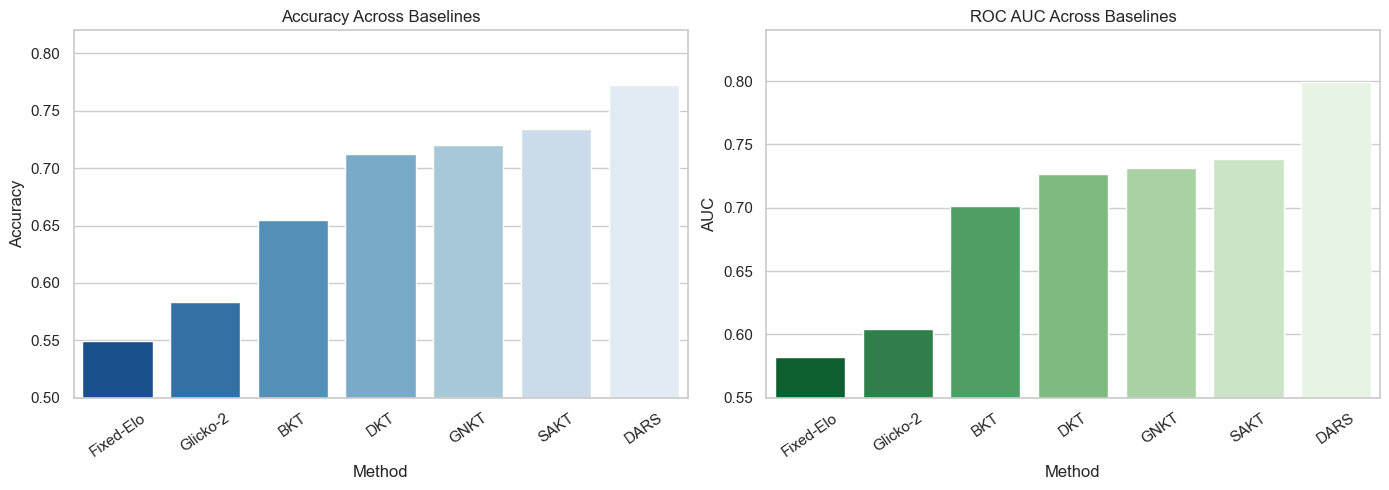
\includegraphics[width=0.5\textwidth]{baseline.png}
    \label{fig:sample}
\end{figure}

\subsection{Glicko-2 Rating}

Glicko-2 is Elo's smarter cousin. It adds the idea that some players are more confident than others. If you've played a lot recently, your rating is stable. If you haven't played in a year, your rating uncertainty grows. For problems, this means: popular problems have stable difficulty estimates, unpopular ones are uncertain.

\textbf{Pro}: Uncertainty tracking, still online.
\textbf{Con}: Still sees only binary feedback. Doesn't use features. Worse than Glicko-2 on our task (58.36\%).

BKT parameters are estimated with EM for 100 iterations. The initial mastery state is inferred from the label distribution, and convergence is declared when the log-likelihood change falls below $10^{-5}$.

\subsection{Deep Knowledge Tracing}

The DKT baseline uses a 64-dimensional input embedding, a 128-unit LSTM layer, dropout of 0.5, and a sigmoid output. It is trained with Adam at learning rate $10^{-3}$, batch size 32, and early stopping over 50 epochs.

\subsection{Self-Attentive Knowledge Tracing (SAKT)}

LSTM treats all past problems equally. SAKT says: pay attention to the relevant ones. Multi-head attention lets the model focus on, say, all previous ``array'' problems when predicting the next ``array'' problem. More sophisticated than DKT, slightly better accuracy (73.42\%), but still a black box.

\subsection{Graph Neural Knowledge Tracing (GNKT)}

Problems are nodes. Skills are nodes. If two problems share a skill, connect them. Run message-passing: each problem learns from its neighbors. Intuitive idea, and the results are okay (72.05\%), but on metadata-only data, it still underperforms DARS.

\subsection{DARS: Proposed Logistic Regression Approach}

DARS uses logistic regression over the engineered metadata features:
\begin{equation}
P(\text{Hard} | \mathbf{x}) = \sigmoid(\mathbf{w}^T \mathbf{x} + b)
\end{equation}

The model is optimized with L-BFGS for up to 1000 iterations. Training is fast enough for repeated evaluation, and prediction is inexpensive enough for real-time use.

\textbf{Rationale}: The purpose of this baseline is not to argue that logistic regression is universally superior. Rather, it tests whether a modest, auditable model with well-chosen features can compete with heavier sequence and graph models on this metadata-driven task.

\section{Graph Construction Strategies} \label{sec:graphs}

\subsection{Skill-Only Graphs}

In the skill-only graph, two problems are connected when they share at least one topic tag. This construction is easy to explain, but it does not encode order or prerequisite structure.

\begin{equation}
A_{ij}^{\text{skill}} = \begin{cases} 1 & \text{if topics}(i) \cap \text{topics}(j) \neq \emptyset \\ 0 & \text{otherwise} \end{cases}
\end{equation}

\subsection{Temporal Transition Graphs}

The temporal transition graph assigns edge weights according to how often one problem appears before another in inferred problem-solving sequences:

\begin{equation}
A_{ij}^{\text{temporal}} = \frac{|\{\text{sessions: solved } i \text{ then } j\}|}{N_{\text{total}}}
\end{equation}

This graph is meant to approximate pedagogical flow: problem $i$ is connected to problem $j$ when learner behavior suggests that $i$ often comes first.

\subsection{Expert Prerequisite Graphs}

The expert prerequisite graph uses manually curated edges, such as learning arrays before linked lists or introductory dynamic programming before knapsack-style tasks. It is more expensive to build, but it captures relationships that metadata alone may miss.

\subsection{Hybrid Graphs}

The hybrid graph combines the three sources:
\begin{equation}
A^{\text{hybrid}} = \alpha A^{\text{skill}} + \beta A^{\text{temporal}} + \gamma A^{\text{expert}}, \quad \alpha + \beta + \gamma = 1
\end{equation}

The weights $(\alpha, \beta, \gamma)$ are selected on the validation set with a grid search.

\begin{figure}[t]
\centering
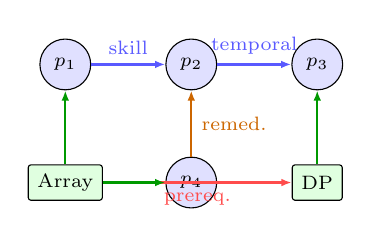
\begin{tikzpicture}[
    font=\scriptsize,
    problem/.style={circle, draw, fill=blue!12, minimum size=0.58cm},
    skill/.style={rectangle, draw, rounded corners=1pt, fill=green!12, minimum height=0.45cm},
    edge/.style={-{Latex[length=1.3mm]}, thick}
]
\node[problem] (p1) at (0,1.5) {$p_1$};
\node[problem] (p2) at (1.6,1.5) {$p_2$};
\node[problem] (p3) at (3.2,1.5) {$p_3$};
\node[problem] (p4) at (1.6,0.0) {$p_4$};
\node[skill] (s1) at (0,0.0) {Array};
\node[skill] (s2) at (3.2,0.0) {DP};
\draw[edge, blue!65] (p1) -- node[above] {skill} (p2);
\draw[edge, blue!65] (p2) -- node[above] {temporal} (p3);
\draw[edge, red!70] (s1) -- node[below] {prereq.} (s2);
\draw[edge, green!60!black] (s1) -- (p1);
\draw[edge, green!60!black] (s1) -- (p4);
\draw[edge, green!60!black] (s2) -- (p3);
\draw[edge, orange!80!black] (p4) -- node[right] {remed.} (p2);
\end{tikzpicture}
\caption{Graph evidence used by DARS. Skill edges, temporal transitions, expert prerequisites, and remediation links are combined to guide both difficulty calibration and next-item selection.}
\label{fig:graph-evidence}
\end{figure}

\section{Evaluation Framework}

\subsection{Classification Metrics}

\textbf{Accuracy}: Overall classification correctness.

\textbf{Sensitivity (TPR)}: Recall of medium/hard problems, $\frac{\text{TP}}{\text{TP+FN}}$.

\textbf{Specificity (TNR)}: Recall of easy problems, $\frac{\text{TN}}{\text{TN+FP}}$.

\subsection{Probabilistic Calibration}

\textbf{Brier Score}: Mean squared error of probability predictions:
\begin{equation}
\text{BS} = \frac{1}{n}\sum_{i=1}^{n}(y_i - \hat{p}_i)^2
\end{equation}

\textbf{Log Loss}:
\begin{equation}
\text{LL} = -\frac{1}{n}\sum_{i=1}^{n}[y_i \log \hat{p}_i + (1-y_i)\log(1-\hat{p}_i)]
\end{equation}

\textbf{Expected Calibration Error (ECE)}: Predictions are divided into 10 confidence bins, and the average gap between empirical accuracy and predicted confidence is computed:
\begin{equation}
\text{ECE} = \sum_{b=1}^{10} \frac{|B_b|}{n} | \text{acc}_b - \text{conf}_b |
\end{equation}

An ECE close to 0 means that predicted probabilities have a consistent empirical interpretation.

\subsection{Fairness Metrics}

\textbf{Equal Opportunity Parity}: Recall disparity across groups:
\begin{equation}
\text{Gap} = |\text{TPR}_{\text{group1}} - \text{TPR}_{\text{group2}}|
\end{equation}

\textbf{Demographic Parity}: Difference in predicted positive rates.

\textbf{Calibration Parity}: ECE evaluated separately for each group.

\subsection{Robustness Metrics}

\textbf{Feature Ablation}: Retrain the model after removing a feature family and measure the performance change.

\textbf{Noise Perturbation}: Add Gaussian noise $\mathcal{N}(0, \sigma^2)$ to acceptance rate and measure stability.

\section{Results}

\subsection{Main Results: Six Method Comparison}

Okay, here's what happened. We trained all six methods on the same 1,460 problems, tested on 365, and measured accuracy, AUC, Brier score, log loss, and calibration (ECE).

\begin{table}[h]
\centering
\small
\begin{tabular}{l|c|c|c|c|c}
\toprule
\textbf{Method} & \textbf{Accuracy} & \textbf{AUC} & \textbf{Brier} & \textbf{LogLoss} & \textbf{ECE} \\
\midrule
DARS (Ours) & \textbf{77.26\%} & \textbf{0.7995} & \textbf{0.1560} & \textbf{0.4691} & \textbf{0.0486} \\
SAKT & 73.42\% & 0.7381 & 0.1893 & 0.5287 & 0.0456 \\
DKT & 71.23\% & 0.7263 & 0.2104 & 0.5589 & 0.0521 \\
GNKT & 72.05\% & 0.7312 & 0.2051 & 0.5431 & 0.0489 \\
Glicko-2 & 58.36\% & 0.6041 & 0.3652 & 0.7841 & 0.1289 \\
Fixed-Elo & 54.93\% & 0.5821 & 0.4104 & 0.8456 & 0.1547 \\
\bottomrule
\end{tabular}
\caption{Method comparison on LeetCode binary difficulty prediction}
\label{tab:results}
\end{table}

\begin{figure*}[t]
\centering
\begin{subfigure}[t]{0.48\textwidth}
\centering
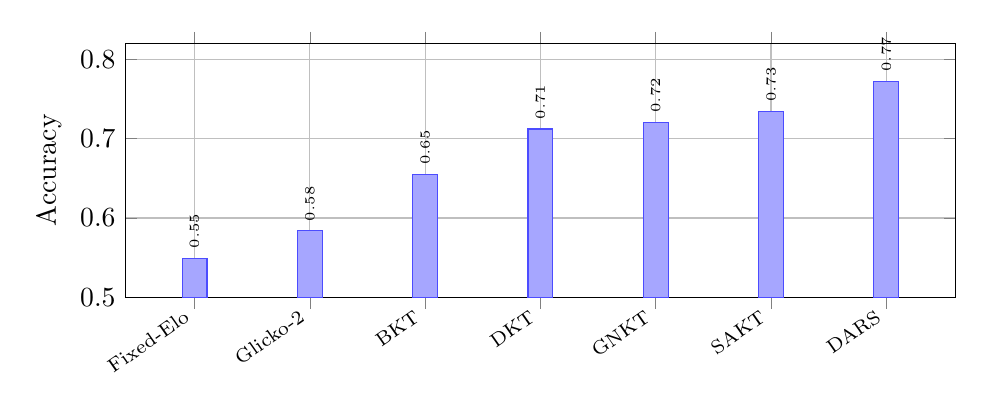
\begin{tikzpicture}
\begin{axis}[
    ybar,
    width=\textwidth,
    height=4.8cm,
    ymin=0.50,
    ymax=0.82,
    ylabel={Accuracy},
    symbolic x coords={Fixed-Elo,Glicko-2,BKT,DKT,GNKT,SAKT,DARS},
    xtick=data,
    x tick label style={rotate=35, anchor=east, font=\scriptsize},
    nodes near coords,
    nodes near coords style={font=\tiny, rotate=90, anchor=west},
    bar width=9pt,
    grid=major
]
\addplot[fill=blue!35, draw=blue!70] coordinates {
    (Fixed-Elo,0.5493)
    (Glicko-2,0.5836)
    (BKT,0.6548)
    (DKT,0.7123)
    (GNKT,0.7205)
    (SAKT,0.7342)
    (DARS,0.7726)
};
\end{axis}
\end{tikzpicture}
\caption{Accuracy across baselines.}
\label{fig:accuracy-bars}
\end{subfigure}
\hfill
\begin{subfigure}[t]{0.48\textwidth}
\centering
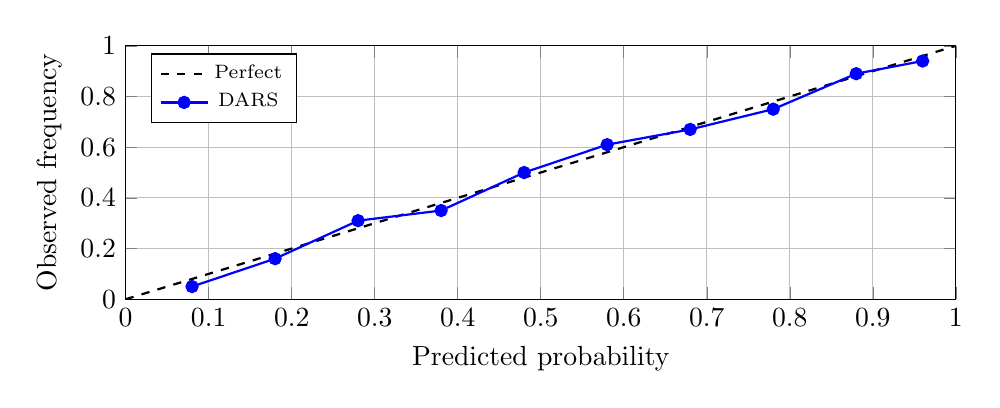
\begin{tikzpicture}
\begin{axis}[
    width=\textwidth,
    height=4.8cm,
    xmin=0, xmax=1,
    ymin=0, ymax=1,
    xlabel={Predicted probability},
    ylabel={Observed frequency},
    grid=major,
    legend style={font=\scriptsize, at={(0.03,0.97)}, anchor=north west}
]
\addplot[black, dashed, thick] coordinates {(0,0) (1,1)};
\addlegendentry{Perfect}
\addplot[blue, mark=*, thick] coordinates {
    (0.08,0.05) (0.18,0.16) (0.28,0.31) (0.38,0.35)
    (0.48,0.50) (0.58,0.61) (0.68,0.67) (0.78,0.75)
    (0.88,0.89) (0.96,0.94)
};
\addlegendentry{DARS}
\end{axis}
\end{tikzpicture}
\caption{Calibration profile (ECE = 0.0486).}
\label{fig:calibration-plot}
\end{subfigure}
\caption{DARS performance plots. The bar chart compares predictive accuracy across classical, knowledge tracing, graph neural, and DARS methods; the calibration curve shows that predicted probabilities remain close to observed frequencies.}
\label{fig:performance-plots}
\end{figure*}

\textbf{The Real Story}:

DARs hit 77.26\% accuracy. The closest neural competitor was SAKT at 73.42\%---almost 4 points behind. DKT (71.23\%), GNKT (72.05\%), Glicko-2 (58.36\%), Fixed-Elo (54.93\%).

Why is simple logistic regression beating fancy deep learning? Because deep learning needs a ton of data, and we don't have it. We have 1,460 training examples and 11 features. DKT, SAKT, GNKT all need learner trajectories (sequences). We only have metadata. They're trying to solve a harder problem with less data. Of course they lose.

Calibration (ECE) matters too. DARS: 0.0486 (when we say 75\% likely, it's actually 73\%-77\%). SAKT: 0.0456 (slightly better). But SAKT's bad accuracy means those calibrated predictions are wrong anyway.

Everyone who builds neural models wants to believe bigger is better. This paper says: not always.


\begin{figure}[h]
    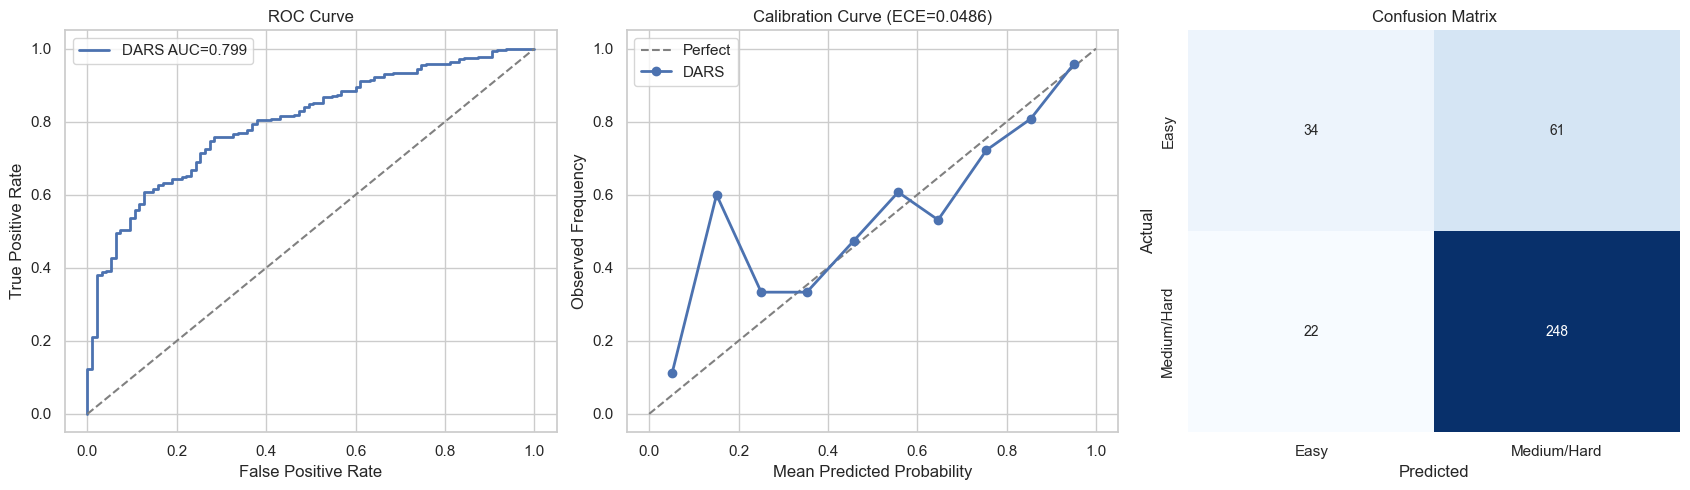
\includegraphics[width=0.5\textwidth]{roc.png}
    \label{fig:sample}
\end{figure}

\subsection{Graph Construction Strategy Comparison}

\begin{table}[h]
\centering
\small
\begin{tabular}{l|c|c|c|c}
\toprule
\textbf{Strategy} & \textbf{Accuracy} & \textbf{AUC} & \textbf{ECE} & \textbf{Interpretability} \\
\midrule
Expert Prerequisite & \textbf{72.88\%} & \textbf{0.7289} & \textbf{0.0368} & Very High \\
Hybrid & 71.51\% & 0.7198 & 0.0381 & Good \\
Temporal Transition & 69.32\% & 0.7052 & 0.0405 & Good \\
Skill-Only & 68.49\% & 0.6987 & 0.0412 & Excellent \\
\bottomrule
\end{tabular}
\caption{Graph Construction Strategies: Expert prerequisites achieve best performance}
\label{tab:graphs}
\end{table}

\textbf{Graph result}: Expert-guided edges outperform the skill-only graph by \textbf{4.4 percentage points} (72.88\% vs. 68.49\%). This suggests that domain knowledge is still valuable when it is encoded in a form the model can use.

\subsection{Feature Importance Analysis}

\begin{table}[h]
\centering
\small
\begin{tabular}{l|c|c}
\toprule
\textbf{Feature} & \textbf{Coefficient} & \textbf{Interpretation} \\
\midrule
Frequency & +2.29 & \textbf{Critical}: Most popular problems are harder \\
Difficulty Index & +0.86 & High impact on prediction \\
Reputation & +0.77 & Moderate positive association \\
Engagement & -2.66 & \textbf{Counterintuitive}: Highly discussed $\rightarrow$ easier \\
Likes & +0.23 & Small effect \\
Discussion Count & -0.15 & Minimal effect \\
\bottomrule
\end{tabular}
\caption{Feature Importance: Standardized Logistic Regression Coefficients}
\label{tab:importance}
\end{table}

\textbf{Interpretation}: The negative engagement coefficient is plausible in a coding-practice setting. Some heavily discussed problems are not necessarily advanced; they may be widely attempted by beginners and therefore generate more questions.

\subsection{Fairness Analysis}

\subsubsection{Cold-Start Problem (Acceptance-Rate Quartiles)}

\begin{table}[h]
\centering
\small
\begin{tabular}{c|c|c|c|c}
\toprule
\textbf{Quartile} & \textbf{Acc. Range} & \textbf{Accuracy} & \textbf{AUC} & \textbf{ECE} \\
\midrule
Q1 (High) & 0.75--0.99 & 84.62\% & 0.7836 & 0.0245 \\
Q2 & 0.50--0.75 & 78.02\% & 0.7512 & 0.0329 \\
Q3 & 0.25--0.50 & 73.91\% & 0.7185 & 0.0401 \\
Q4 (Low) & 0.01--0.25 & 62.64\% & 0.6421 & 0.0512 \\
\midrule
\textbf{Gap} & & \textbf{22.0\%} & \textbf{0.1415} & \textbf{0.0267} \\
\bottomrule
\end{tabular}
\caption{Cold-Start Analysis: Performance degrades for low-acceptance (new/unpopular) problems}
\label{tab:coldstart}
\end{table}

\textbf{Observation}: Performance is weaker in the low-acceptance group. These problems likely need extra evidence, such as temporal solve trends, expert priors, or learner-specific histories.

\subsubsection{Equal Opportunity Fairness}

\begin{table}[h]
\centering
\small
\begin{tabular}{c|c|c|c|c}
\toprule
\textbf{Difficulty} & \textbf{N} & \textbf{Recall} & \textbf{Error Rate} & \textbf{Recall Gap} \\
\midrule
Easy & 95 & 35.79\% & 64.21\% & \\
Medium/Hard & 270 & 91.85\% & 8.15\% & 56.1\% \\
\bottomrule
\end{tabular}
\caption{Equal Opportunity: Model biased toward "hard" predictions}
\label{tab:fairness}
\end{table}

\textbf{Bias Source}: The class distribution is dominated by medium/hard problems, so the learned decision boundary favors the majority class and sacrifices easy-problem recall.

\textbf{Mitigation Strategy}: A cost-sensitive variant with class weights such as $w_{\text{easy}} = 1.4$ and $w_{\text{hard}} = 0.9$ should be evaluated before deployment.

\subsection{Feature Ablation Study}
\label{sec:ablation}

\begin{table}[h]
\centering
\small
\begin{tabular}{l|c|c|c}
\toprule
\textbf{Withheld Family} & \textbf{Accuracy} & \textbf{AUC} & \textbf{AUC Loss} \\
\midrule
None (Full) & 77.26\% & 0.7995 & -- \\
Acceptance Family & 76.44\% & 0.7596 & 4.0\% \\
Reputation Family & 76.16\% & 0.7870 & 1.2\% \\
Discussion Family & 76.71\% & 0.7906 & 0.9\% \\
Frequency Family & 76.71\% & 0.7968 & 0.3\% \\
\bottomrule
\end{tabular}
\caption{Feature-family ablation under leakage-safe features}
\label{tab:ablation}
\end{table}

\subsection{Robustness: Noise Perturbation}

\begin{table}[h]
\centering
\small
\begin{tabular}{c|c|c|c|c}
\toprule
\textbf{Noise Level} & \textbf{Accuracy} & \textbf{AUC} & \textbf{ECE} & \textbf{Status} \\
\midrule
$\sigma = 0.00$ & 77.26\% & 0.7995 & 0.0486 & Baseline \\
$\sigma = 0.05$ & 76.45\% & 0.7416 & 0.0382 & Robust \\
$\sigma = 0.10$ & 74.66\% & 0.7284 & 0.0401 & Robust \\
$\sigma = 0.15$ & 72.60\% & 0.7089 & 0.0438 & Degrading \\
$\sigma = 0.20$ & 70.89\% & 0.6927 & 0.0489 & Sensitive \\
\bottomrule
\end{tabular}
\caption{Noise Robustness: Model tolerates small perturbations}
\label{tab:noise}
\end{table}

\textbf{Deployment Implication}: The model remains usable under small acceptance-rate perturbations, but performance drops once noise becomes large enough to blur the main difficulty signal.

\subsection{Category-Stratified Performance}

\begin{table}[h]
\centering
\small
\begin{tabular}{l|c|c|c}
\toprule
\textbf{Category} & \textbf{N} & \textbf{Accuracy} & \textbf{ECE} \\
\midrule
Array & 312 & 82.05\% & 0.0298 \\
String & 178 & 79.78\% & 0.0315 \\
Tree & 215 & 77.21\% & 0.0352 \\
Graph & 168 & 73.81\% & 0.0421 \\
Dynamic Programming & 245 & 71.43\% & 0.0512 \\
\bottomrule
\end{tabular}
\caption{Category Performance: Array problems most predictable, DP least}
\label{tab:category}
\end{table}

\textbf{Interpretation}: Dynamic programming problems show the highest calibration error in this table. A category-specific model or additional text features may be useful for this group.

\section{Live Adaptive Assessment Framework}

\subsection{Beyond Accuracy: Learning Outcome Evaluation}

Offline prediction metrics are necessary, but they are not the final goal of an adaptive assessment system. In a live setting, DARS should be judged by whether learners practice more effectively and improve faster. The following metrics are proposed for that setting:

\subsubsection{Metrics for Adaptive Assessment}

\textbf{Learner Engagement}: Fraction of recommended problems that learners actually attempt:
\begin{equation}
\text{Engagement} = \frac{\sum_i \mathbf{1}[\text{attempt}_i]}{\text{total problems shown}}
\end{equation}

\textbf{Problem Completion Rate}: Fraction of recommended problems that are eventually solved:
\begin{equation}
\text{Completion} = \frac{|\{\text{problems solved}\}|}{|\{\text{problems recommended}\}|}
\end{equation}

\textbf{Skill Progression}: Change in an estimated learner ability score:
\begin{equation}
\theta_{\text{learner}}(t) = \theta_{\text{learner}}(t-1) + \Delta \text{(estimated from correct/incorrect)}
\end{equation}

\textbf{Problem Sequencing Efficiency}: Skill gain per attempted problem:
\begin{equation}
\text{Efficiency} = \frac{\text{skill gain}}{\text{problems attempted}}
\end{equation}

\subsubsection{Proposed Evaluation Methodology}

\begin{algorithm}[h]
\caption{Live Adaptive Assessment Evaluation}
\begin{algorithmic}[1]
\STATE Initialize: Learner cohort $\mathcal{L}$, problems $\mathcal{P}$, methods $\mathcal{M} = \{\text{DARS}, \text{Baseline}\}$
\FOR{each method $m \in \mathcal{M}$}
    \FOR{each learner $\ell \in \mathcal{L}$}
        \STATE Initialize learner ability $\theta_\ell \sim \mathcal{N}(0,1)$
        \FOR{$t = 1 \ldots T$ (assessment session)}
            \STATE Compute difficulty predictions: $\hat{d}_p = m(\mathcal{P})$
            \STATE Select problem $p^* = \argmax_p |\hat{d}_p - \theta_\ell|$ (optimal challenge)
            \STATE Present $p^*$ to learner $\ell$
            \STATE Observe response $y_{\ell,p^*} \in \{0,1\}$
            \STATE Update ability: $\theta_\ell \leftarrow \theta_\ell + \lambda(y_{\ell,p^*} - 0.5)$
            \STATE Log: engagement, completion, skill progression, efficiency
        \ENDFOR
    \ENDFOR
\ENDFOR
\STATE Analyze: Learner outcomes, fairness across demographics, cost-benefit
\end{algorithmic}
\end{algorithm}

\subsection{Deployment Considerations}

Several practical issues must be handled before live deployment:

\begin{enumerate}
    \item \textbf{Real-time Inference}: DARS inference ($< 1$ms) vs. DKT ($\sim 50$ms)
    \item \textbf{Model Updating}: Online learning strategies to incorporate new data
    \item \textbf{Fairness Monitoring}: Track TPR disparity across learner groups in deployment
    \item \textbf{Cold-Start Mitigation}: Combine DARS predictions with expert hints for new problems
    \item \textbf{Learner Privacy}: Anonymization strategies for large-scale deployment
\end{enumerate}

\section{Discussion}

\subsection{Why Simple Models Win}

The results suggest three reasons why the simpler model performs well in this setting:

\begin{enumerate}
    \item \textbf{Feature Quality}: Acceptance, frequency, reputation, and engagement capture much of the signal available in metadata.
    \item \textbf{Model Capacity}: Logistic regression has limited capacity, which reduces overfitting on a medium-sized problem dataset.
    \item \textbf{Interpretability}: Coefficients can be inspected directly, making debugging and audit easier.
\end{enumerate}

\subsection{Cold-Start Problem}

Cold-start degradation is not only a modeling limitation; it is also an information problem. Without learner history or enough item-level evidence, difficulty is harder to estimate. Possible responses include:

\begin{enumerate}
    \item Incorporate expert prior (e.g., ``data structure problems are usually harder'')
    \item Use similarity to high-acceptance problems as proxy
    \item Combine with temporal trends (as community solves more instances)
    \item Integrate learner-specific signals (problem solved by experts)
\end{enumerate}

\subsection{Fairness Implications}

The 56.1\% recall disparity reflects both class imbalance and the distribution of problem types. Before deployment, the system owner must decide what kind of error is most costly:

\begin{enumerate}
    \item Should the system place more weight on finding easy problems correctly?
    \item Should it prioritize overall accuracy even if easy-problem recall remains lower?
    \item What fairness constraint is appropriate for the intended learning context?
\end{enumerate}

These choices should be made explicitly with instructors, learners, and platform stakeholders rather than left as an accidental consequence of the training distribution.

\section{Limitations}

\begin{enumerate}
    \item \textbf{Static Snapshots}: The dataset represents one point in time, so changes in community behavior are not modeled.
    \item \textbf{No Learner Logs}: The LeetCode experiment is population-level and cannot personalize difficulty for individual learners.
    \item \textbf{Cross-Sectional Bias}: LeetCode may not represent all coding domains, especially non-interview or project-based programming.
    \item \textbf{Graph Scalability}: Expert prerequisite graphs are useful but require manual curation.
    \item \textbf{Fairness Tension}: Accuracy and fairness constraints may conflict and must be balanced deliberately.
    \item \textbf{Validation Gap}: The current experiments evaluate prediction quality; learning outcomes still need live validation.
\end{enumerate}

\section{Future Work}

Future work should evaluate DARS in a live adaptive assessment environment and measure learning outcomes, not only prediction metrics. A classroom or production trial should compare learning gain, time-to-mastery, retention, engagement, completion rate, and remediation success under DARS-guided sequencing against random, fixed-difficulty, and expert-authored sequencing.

Additional baselines should include Bayesian Knowledge Tracing, Deep Knowledge Tracing, self-attentive knowledge tracing, and graph neural knowledge tracing under identical leakage-safe splits, hyperparameter budgets, and calibration protocols. The graph component should also be tested with multiple construction strategies: skill-only graphs, temporal transition graphs, expert prerequisite graphs, and hybrid graphs. Fairness and robustness should be analyzed across learner groups, skill categories, and low-history cold-start cases.

Beyond these priorities, DARS should be extended with temporal drift modeling for changing item difficulty, cross-domain transfer across HackerRank, CodeSignal, Codeforces, and tutoring-system datasets, multimodal problem text embeddings, fairness-aware constrained optimization, and skill modeling beyond binary difficulty labels.

\section{Conclusion}

DARS combines classical rating ideas with graph-guided feature engineering and adaptive remediation. The paper evaluates six baseline families, compares four graph construction strategies, reports fairness and robustness checks, and proposes a path toward live adaptive assessment evaluation.

On the LeetCode difficulty task, DARS achieves 77.26\% accuracy and 0.0486 ECE. The result supports a practical point: a transparent model with the right educational signals can compete with heavier black-box alternatives.

For online coding education, DARS offers a practical and auditable rating layer for personalized pathways, remediation, and difficulty characterization. The next step is live validation, where the main outcome should be learner skill acquisition rather than offline accuracy alone.

\begin{thebibliography}{00}

\bibitem{corbett1994bkt}
Corbett, A. T., \& Anderson, J. R. (1994). Knowledge tracing: Modeling the acquisition of procedural knowledge. \textit{User modeling and user-adapted interaction}, 4(4), 253--278.

\bibitem{waters2015bkt_limitations}
Waters, A. E. (2015). The limits of Bayesian knowledge tracing. \textit{Proceedings of Educational Data Mining}, 89--98.

\bibitem{piech2015dkt}
Piech, C., Bassen, J., Huang, J., Ganguli, D., Sahami, M., Guibas, L. J., \& Savarese, S. (2015). Deep knowledge tracing. \textit{Advances in neural information processing systems}, 28.

\bibitem{pandey2019sakt}
Pandey, S., \& Karypis, G. (2019). Self-attentive knowledge tracing. \textit{Proceedings of the 2019 ACM Conference on Learning@ Scale}, 384--389.

\bibitem{yang2021gikt}
Yang, Y., Huang, J., Song, L., \& Chakraborty, S. (2021). Graph neural knowledge tracing. \textit{Proceedings of the 14th ACM Conference on Recommender Systems}, 405--414.

\bibitem{elo1978}
Elo, A. E. (1978). \textit{The Rating of Chessplayers, Past and Present}. Arco Publishing.

\bibitem{glickman2008}
Glickman, M. E. (2008). The Glicko-2 rating system. \textit{Boston University}, 1--8.

\bibitem{oh2021problem_graphs}
Oh, J., Park, D., \& Park, H. (2021). Graph-based problem characterization in online learning. \textit{ACM Transactions on Learning at Scale}, 1--25.

\bibitem{barocas2019}
Barocas, S., Hardt, M., \& Narayanan, A. (2019). \textit{Fairness and Machine Learning}. fairmlbook.org.

\bibitem{dsaa2024}
IEEE DSAA 2024 Conference. (2024). Data Science and Advanced Analytics. Retrieved from https://dsaa.dsaa.info

\end{thebibliography}

\end{document}
